% !TEX root = ./Basilisk-ThrusterForces-20160627.tex

\section{Test Description and Success Criteria}
The module is run with 5 parameters:
\begin{enumerate}
\item useDVThruster: Determines if using a DV thruster configuration or a RCS thruster configuration
\item useCOMOffset: Offset the COM from the control axes. 
\item dropThruster: Removes 2 of the 6 original thrusters within the DV configuration, or 1 of the 8 in the RCS configuration.
\item dropAxis: Removes 1 of the 3 control axes in the RCS configuration.
\item saturateThrusters: Changes the angle tolerance which triggers scaling behavior.
\end{enumerate}

\subsubsection{ACS Thruster Configuration}
To illustrate the performance of this algorithm, the following simulation setup is used.  Let the ACS system have a total of $N = 8$ thrusters with the following body-fixed locations:
\begin{gather*}
	\label{eq:th:loc}
	\bm r_{1} = \begin{bmatrix} +1.125, 0.0, +0.75  \end{bmatrix}^{T} \text{ m}
	\quad\quad
	\bm r_{2} = \begin{bmatrix} -1.125, 0.0, +0.75  \end{bmatrix}^{T} \text{ m}
	\\
	\bm r_{3} = \begin{bmatrix} -1.125, 0.0, +0.75  \end{bmatrix}^{T}	 \text{ m}
	\quad\quad
	\bm r_{4} = \begin{bmatrix} +1.125, 0.0, +0.75  \end{bmatrix}^{T} \text{ m}
	\\
	\bm r_{5} = \begin{bmatrix} +1.125, 0.0, -0.75  \end{bmatrix}^{T}	 \text{ m}
	\quad\quad
	\bm r_{6} = \begin{bmatrix} -1.125, 0.0, -0.75  \end{bmatrix}^{T} \text{ m}
	\\
	\bm r_{7} = \begin{bmatrix} -1.125, 0.0, -0.75  \end{bmatrix}^{T}	 \text{ m}
	\quad\quad
	\bm r_{8} = \begin{bmatrix} +1.125, 0.0, -0.75  \end{bmatrix}^{T} \text{ m}
\end{gather*}
with the force unit direction vectors:
\begin{gather*}
	\label{eq:th:gt}
	\bm g_{t_{1}} = \begin{bmatrix} +0.707107, +0.707107, 0  \end{bmatrix}^{T}
	\quad\quad
	\bm g_{t_{2}} = \begin{bmatrix} -0.707107, +0.707107, 0  \end{bmatrix}^{T}
	\\
	\bm g_{t_{3}} = \begin{bmatrix} -0.707107, -0.707107, 0  \end{bmatrix}^{T}
	\quad\quad
	\bm g_{t_{4}} = \begin{bmatrix} +0.707107, -0.707107, 0  \end{bmatrix}^{T}
	\\
	\bm g_{t_{5}} = \begin{bmatrix} +0.707107, +0.707107, 0 \end{bmatrix}^{T}
	\quad\quad
	\bm g_{t_{6}} = \begin{bmatrix} -0.707107, +0.707107, 0  \end{bmatrix}^{T}
	\\
	\bm g_{t_{7}} = \begin{bmatrix} -0.707107, -0.707107, 0  \end{bmatrix}^{T}
	\quad\quad
	\bm g_{t_{8}} = \begin{bmatrix} +0.707107, -0.707107, 0  \end{bmatrix}^{T}
\end{gather*}
\begin{figure}[htb]
	\centerline{
	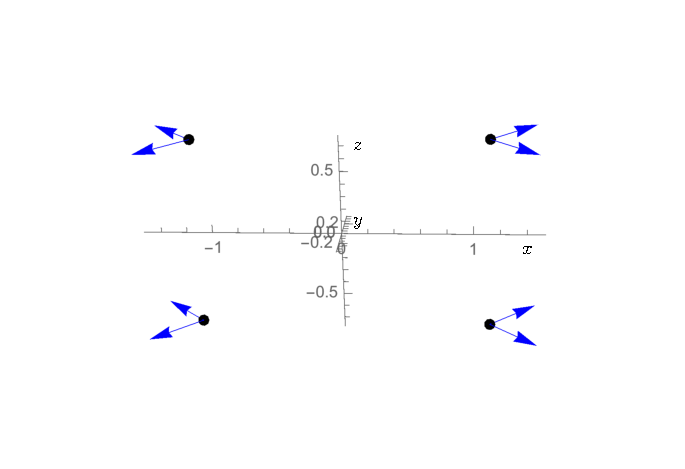
\includegraphics[]{Figures/8ThrConfig}
	}
	\caption{Illustration of an 8-thruster ACS configuration}
	\label{fig:8ThrConfig}
\end{figure}
\begin{figure}[p]
	\centering
	\subfigure[Percent Torque Error]
	{\label{fig:minTorquePer}
	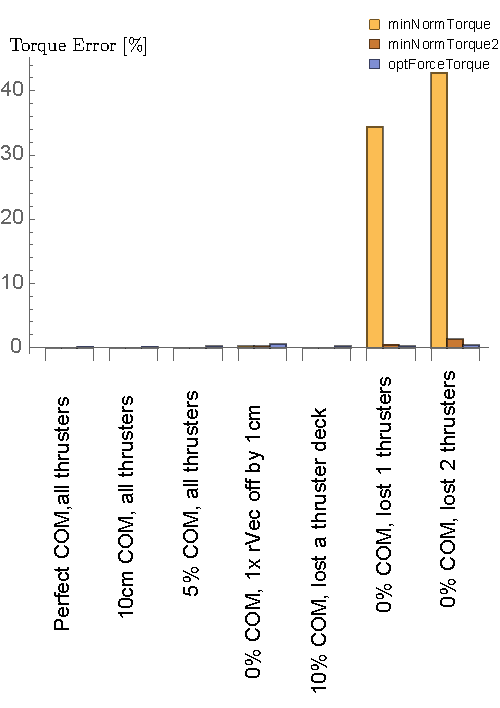
\includegraphics[width=0.45\textwidth]{Figures/minTorquePer}} 
	\\
	\subfigure[Thruster Control Implementation Effort]
	{\label{fig:minTorqueSumF} 
	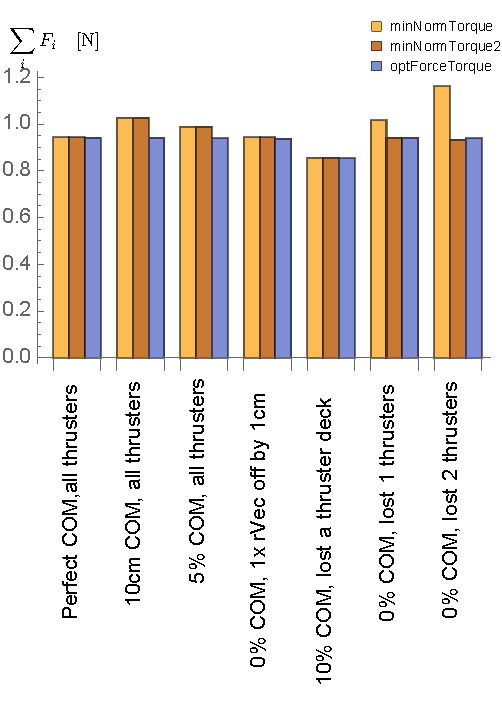
\includegraphics[width=0.45\textwidth]{Figures/minTorqueSumF}}  
	\subfigure[Net Thruster Disturbance Force]
	{\label{fig:minTorqueNetF} 
	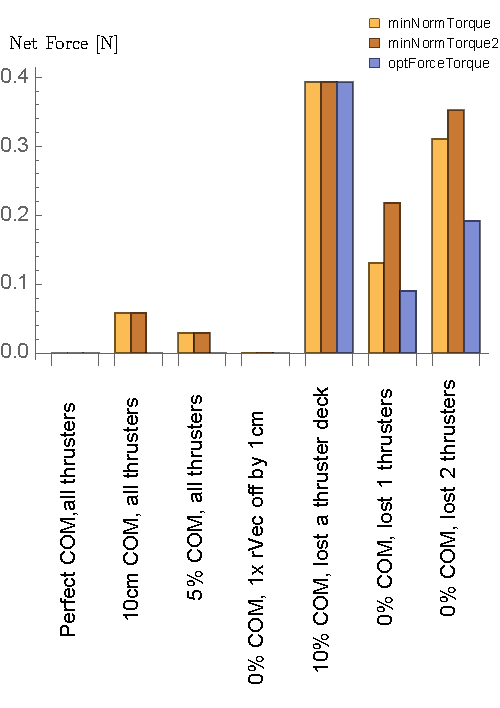
\includegraphics[width=0.45\textwidth]{Figures/minTorqueNetF}}  
	\caption{ACS Thruster Mapping Performance Mapping Illustration Comparing the 1-stage and 2-stage minimum norm solution to the thruster mapping of a nonlinear optimization solution.}
	\label{fig:minTorque}
\end{figure}


The resulting configuration is illustrated in Figure~\ref{fig:8ThrConfig}.  In this setup the center of mass position vector is set to $\bm r_{\text{COM}} = (0,0,0)^{T} \text{ m}$.  The following plots show the thruster firing performance by considering a rang of scenarios.  The first case assumes all thrusters are available, and the $\bm r_{\text{COM}}$ vector is known perfectly.  The second and third case also have all thrusters available, but the $\bm r_{\text{COM}}$ vector knowledge is off by 10cm or 5cm in the $z$ direction.  The 4th case has the perfect $\bm r_{\text{COM}}$ vector, but the first thruster location is off by 1cm in the $y$ direction.  The 5th case again assumes a 10cm COM offset, but also that only 4/8 thrusters are available.  In essence, all the lower or upper thruster have become un-available.  The 6th and 7th case assumes perfect COM knowledge, but either the last one or last two thrusters are un-available.  


The resulting performance is illustrated in Figure~\ref{fig:minTorque}.  Here 20 random $\bm L_{r}$ torques are generated, and the mean results are shown.  The $[C]$ matrix is set to the identity matrix to control all three axes.   The 1-stage minimum norm algorithm is compared to an optimal thruster firing solution which minimizes the net thruster forces used, the net disturbance torque onto the craft, all subject to producing the desired control torque.    Regarding generating the desired control torque, only when 1 or 2 thrusters were lost did the algorithm have issues generating the required torque.  In all other cases the desired torque was always produced as shown in Figure~\ref{fig:minTorquePer}.  In comparison, the 2-stage minimum norm algorithm performs very well in these latter cases where 1-2 thrusters are lost, yielding only very small torque errors on average.  

The control effort required to achieve this torque is shown in Figure~\ref{fig:minTorqueSumF}.  Here the $F_{i}$ thruster force values are simply summed to have a sense of how much on-time or fuel is required for a given scenario.  If all ACS thrusters are operating and the COM is perfectly modeled is the control effort equivalent to the optimal solution.  In all other case the effort is about 10-20\% larger.  in contrast, the 2-stage minimum norm algorithm control efforts in the cases with lost thrusters is very similar to those of the optimal answers.  This illustrates the robustness achieved by adding this 2nd stage if some thrusters are lost.  

Finally, to see how well this algorithm is able to avoid net disturbance forces onto the spacecraft, the results in Figure~\ref{fig:minTorqueNetF} are shown.  Overall the 1-stage algorithm did well, producing 0 net force in the ideal case and the case where the 1st thruster location is different, and matches the optimal answer for the lost thruster deck and lost single thruster case.  In the other cases there is some net disturbance force.  The 2-stage algorithm only differs here when thrusters are lost.  Here the net disturbance torque is higher than the 1-stage solution.  However, this is an expected result as the 1-stage solution produces huge torque errors, while the 2-stage solution produces a very different thruster solution which yields very small torque errors. 

Overall the 2-stage thruster firing performs very well in comparison to the the optimal thruster firing solutions.  The optimal solutions are computationally very expensive and not suitable to realtime flight-software implementations.  








\subsubsection{DV Thruster Configuration}
Next consider a DV thruster configuration where the off-thruster-axis control torques are produces through off-pulsing.  Let the DV system have a total of $N = 6$ thrusters with the following body-fixed locations:
\begin{align*}
	\label{eq:th:loc}
	\bm r_{1} &= \begin{bmatrix} 0, 0.413, -0.1671  \end{bmatrix}^{T} \text{ m}
	& 
	\bm r_{2} &= \begin{bmatrix} 0.357668, 0.2065, -0.1671  \end{bmatrix}^{T} \text{ m}
	\\
	\bm r_{3} &= \begin{bmatrix} 0.357668, -0.2065, -0.1671 \end{bmatrix}^{T}	 \text{ m}
	&
	\bm r_{4} &= \begin{bmatrix} 0, -0.413, -0.1671  \end{bmatrix}^{T} \text{ m}
	\\
	\bm r_{5} &= \begin{bmatrix} -0.357668, -0.2065, -0.1671  \end{bmatrix}^{T}	 \text{ m}
	&
	\bm r_{6} &= \begin{bmatrix} -0.357668, 0.2065, -0.1671 \end{bmatrix}^{T} \text{ m}
\end{align*}
with the force unit direction vectors given by $\hat{\bm g}_{t_{i}} = (0,0,1)^{T}$ as illustrated in Figure~\ref{fig:6ThrConfig}.
\begin{figure}[t]
	\centerline{
	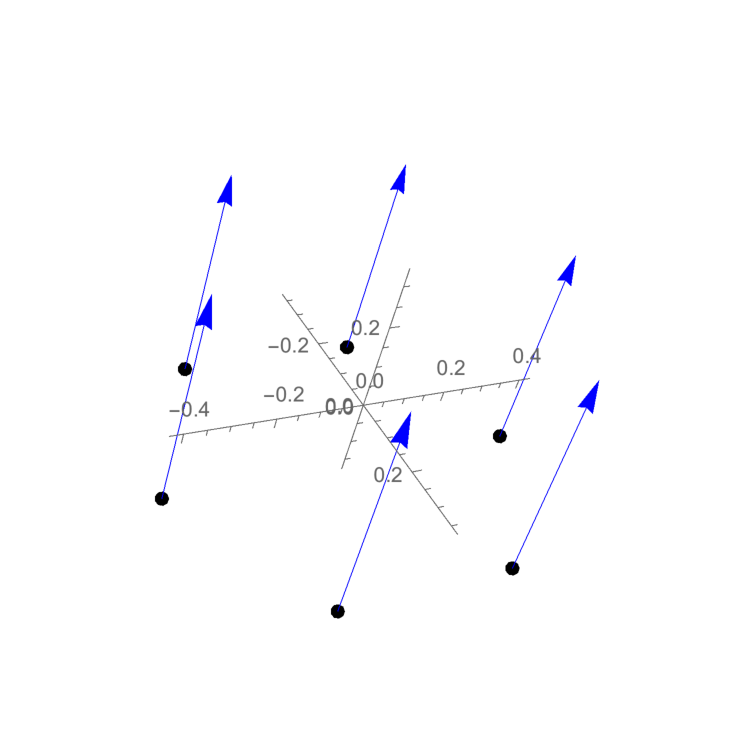
\includegraphics[width=0.4\textwidth]{Figures/dvThrConfig}
	}
	\caption{Illustration of an 6-thruster DV configuration}
	\label{fig:6ThrConfig}
\end{figure}


\begin{figure}[t]
	\centering
	\subfigure[Percent Torque Error]
	{\label{fig:minTorquePerDV}
	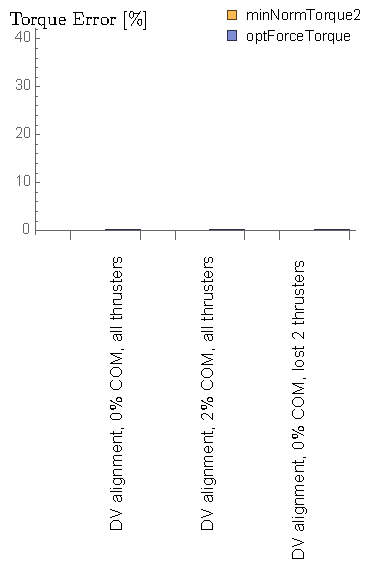
\includegraphics[width=0.4\textwidth]{Figures/dvTorquePer}} 
	\subfigure[Thruster Control Implementation Effort]
	{\label{fig:minTorqueSumFDV} 
	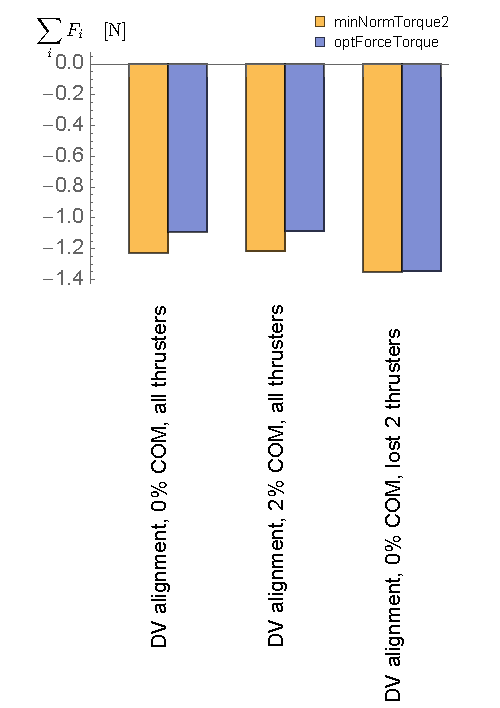
\includegraphics[width=0.45\textwidth]{Figures/dvSumF}}  
	\caption{DV Thruster Mapping Performance Mapping Illustration Comparing the 1-stage and 2-stage minimum norm solution to the thruster mapping of a nonlinear optimization solution.}
	\label{fig:minTorqueDV}
\end{figure}

Figure~\ref{fig:minTorqueDV} illustrates the DV off-pulsing performance for 3 scenarios.  The 1st one has all thrusters available and no COM error.  The 2nd case adds 2cm COM offsets to the $x$ and $y$ axes, while the 3rd case has no COM error but lost an opposing set of thrusters.  Again 20 random $\bm L_{r}$ vectors are generated and the mean performance evaluated.  As only torques about the $x$ and $y$ axis can be controlled with this DV thruster configuration, the control axis matrix is set to 
$$
	[C] = \begin{bmatrix}
		1 & 0 & 0 \\
		0 & 1 & 0
	\end{bmatrix}
$$

The torque implementation errors are compared in Figure~\ref{fig:minTorquePerDV}.  The 2-stage process outlined above is able to produce the required torques in all cases, illustrating good robustness to COM offsets and loosing 2/6 thrusters.  Figure~\ref{fig:minTorqueSumFDV} illustrates the net off-pulsing effort required to achieve these random control torque vectors.  The 2-stage algorithms requires slightly more off-pulsing than the optimal solution.  However, the difference isn't very large, especially in comparison to the drastically faster computational evaluation time.  



\section{Test Parameters}


\begin{table}[htbp]
	\caption{Error tolerance for each test.}
	\label{tab:errortol}
	\centering \fontsize{10}{10}\selectfont
	\begin{tabular}{ c | c } % Column formatting, 
		\hline\hline
		\textbf{Output Value Tested}  & \textbf{Tolerated Error}  \\ 
		\hline
		{\tt motorTorque}        & 	  1e-05 \\ 
		\hline\hline
	\end{tabular}
\end{table}




\section{Test Results}

All of the tests passed:
\begin{table}[H]
	\caption{Test results}
	\label{tab:results}
	\centering \fontsize{10}{10}\selectfont
	\begin{tabular}{c | c  |c | c |c |c} % Column formatting, 
		\hline\hline
		\textbf{DVThruster?} & 	\textbf{useCOMOffset?}	& \textbf{dropThrusters}	  & \textbf{dropAxis?}		& \textbf{saturateThrusters} &\textbf{Pass/Fail} \\ 
		\hline
	   	   			False &  False & False & False & 0 & \input{AutoTeX/passFail_False_False_False_False_0.tex}\\ 
	   	   			False &  False & False & False & 1 & \input{AutoTeX/passFail_False_False_False_False_1.tex}\\ 
	   	   			False &  False & False & False & 2 & \input{AutoTeX/passFail_False_False_False_False_2.tex}\\ 
	   	   			False &  False & False & False & 3 & \input{AutoTeX/passFail_False_False_False_False_3.tex}\\ 
	   	   			False &  False & False & True & 0 & \input{AutoTeX/passFail_False_False_False_True_0.tex}\\ 
	   	   			False &  True & False & False & 0 & \input{AutoTeX/passFail_False_True_False_False_0.tex}\\ 
	   	   			True &  False & False & False & 0 & \input{AutoTeX/passFail_True_False_False_False_0.tex}\\ 
	   	   			True &  False & False & False & 1 & \input{AutoTeX/passFail_True_False_False_False_1.tex}\\ 
	   	   			True &  False & False & False & 2 & \input{AutoTeX/passFail_True_False_False_False_2.tex}\\ 
	   	   			True &  False & True & False & 0 & \input{AutoTeX/passFail_True_False_True_False_0.tex}\\ 
	   	   			True &  True & False & False & 0 & \input{AutoTeX/passFail_True_True_False_False_0.tex}\\ 
	   \hline\hline
	\end{tabular}
\end{table}





